    \section{Scenarios and results}
    The project is about sentiment analysis of people's attitudes toward the current COVID-19 pandemic. Four scenarios are covered, for each SA4 area, the project analyses how many COVID related tweets are posted, people's attitudes toward the mobile application, COVIDSafe. And generally, the most common COVID symptoms, the number of tweets mention the symptoms in three major cities, Melbourne, Sydney and Perth.
    
    The analysis is proceed based on the tweets in Australia collected by the harvester, the analyses below are based on 5.5 millions COVID related tweets, 30K tweets about COVID symptoms and 25K about covidsafe.
    
    \subsection{Count of COVID Related Tweets for Each SA4 Area}
    
    The overall result does not show much valuable information. Tweets are concentrating on the major cities but suddenly decrease to relative low numbers in the other areas. 
    
    \begin{figure}[H]
    \centering
    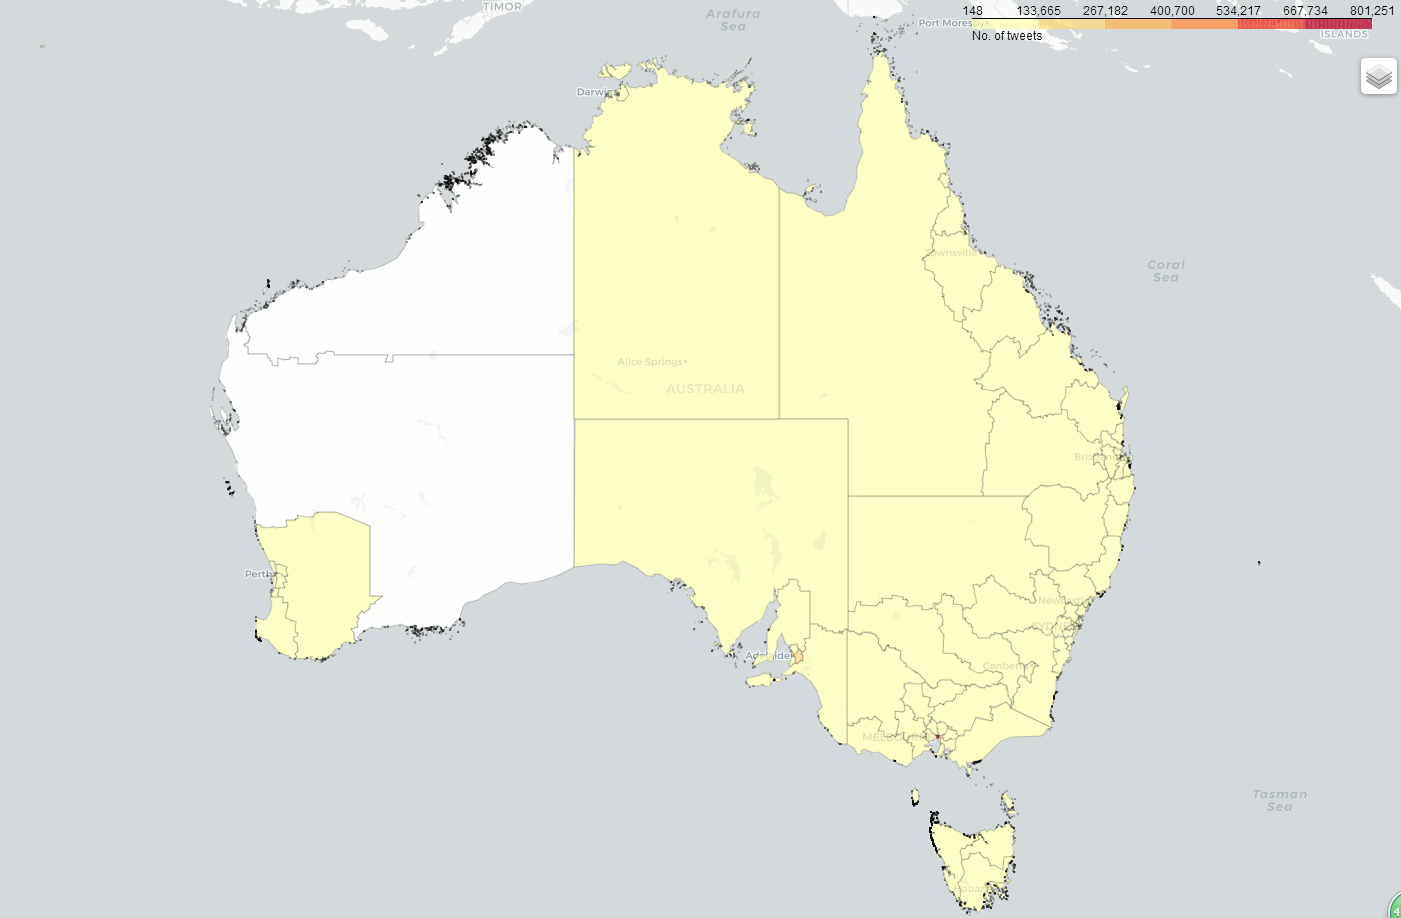
\includegraphics[scale=0.35]{city_analytics/report/images/covidtweet.png}
    \caption{Number of COVID tweets for each SA4}
    \label{fig:Number of COVID tweets for each SA4}
    \end{figure}
    
    The reason is the majority of tweets do not have exact geo coordinates, thus, the SA4 codes for them come from matching the city name with our defined city name to SA4 dictionary. However, Twitter does not provide detailed city names, city names are given in a broader range, so matching name to SA4 has a relative low accuracy, for instance, SA4 area Inner Melbourne, East Melbourne may all provided as Melbourne which results in the data peaks at Melbourne but low in other areas.
    
    \begin{figure}[H]
    \centering
    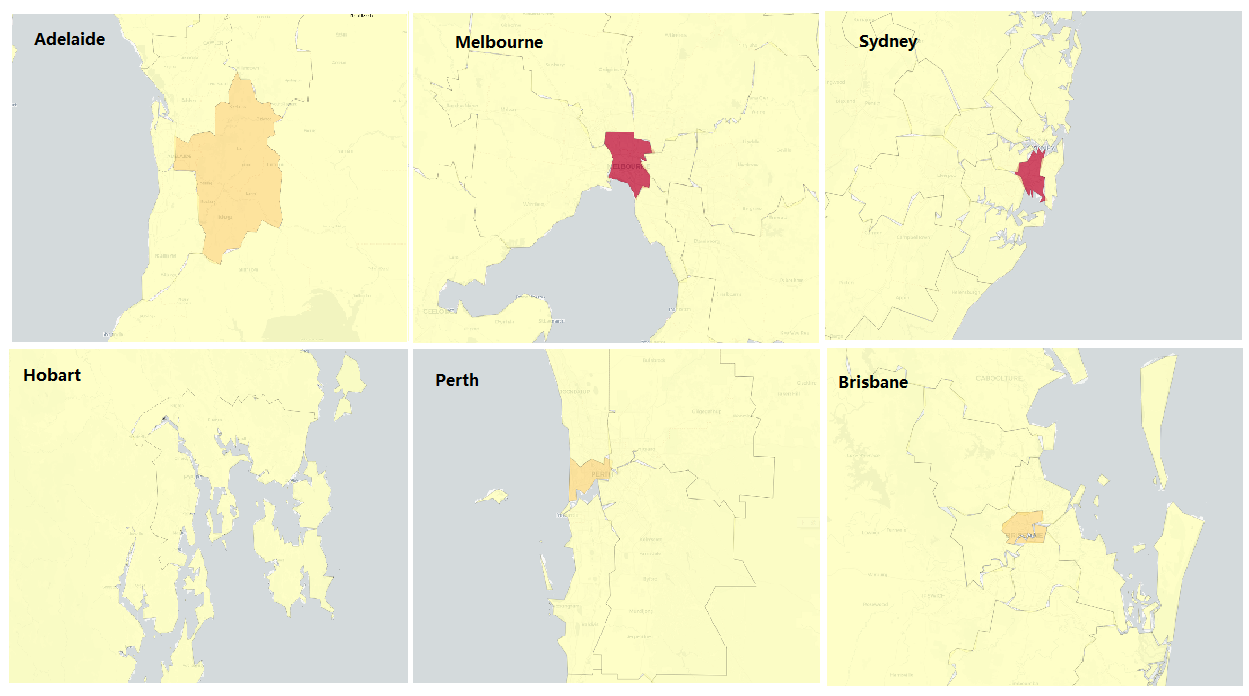
\includegraphics[scale=0.4]{city_analytics/report/images/covid-tweets-each-city.png}
    \caption{Number of COVID tweets for major cities}
    \label{fig:Number of COVID tweets for major cities}
    \end{figure}
    
    \subsection{Attitude related to the COVIDSafe app} 
    Compared with previous quantity based analysis, a ratio based analysis can tell much more.The scenario is analysing people's attitudes toward the mobile application, COVIDSafe. The ratio is calculated as
    
    \[\frac{\text{number of positive tweets}}{\text{negative} + \text{positive}}\]
    The first impression given by this graph is green, which indicates that people are generally optimistic about the software, and only a few areas show people's concerns. This optimism might because Australia has well controlled the epidemic, and did not cause widespread spread of the virus, people do not have much worry about the pandemic.
   
    \begin{figure}[H]
    \centering
    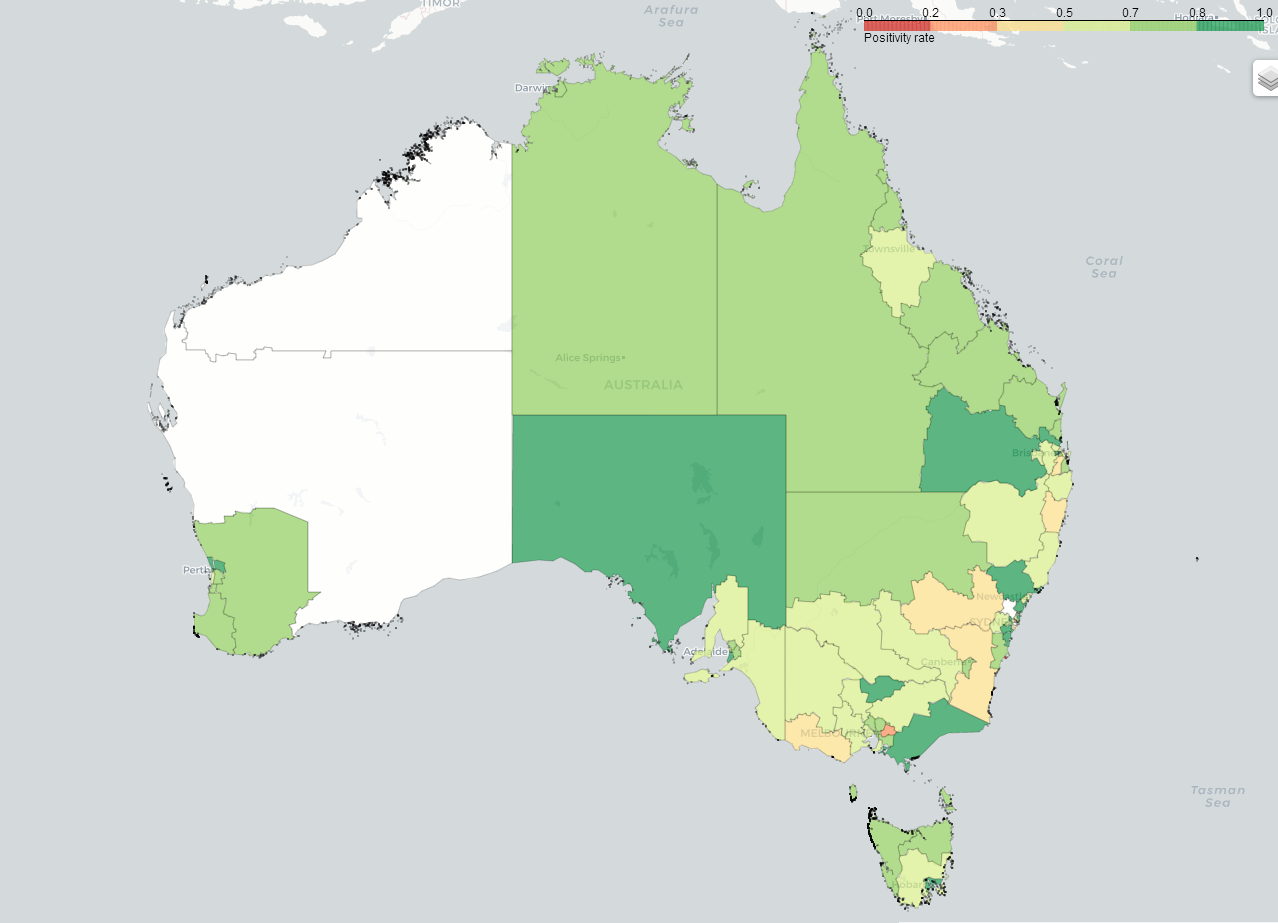
\includegraphics[scale=0.4]{city_analytics/report/images/covidsafe.png}
    \caption{Attitude related to the COVIDSafe app}
    \label{fig:Attitude related to the COVIDSafe app}
    \end{figure}
    
    \subsection{Most Common COVID Symptoms}
    
    This picture intuitively shows the most common symptoms of COVID-19 are fever, cough, fatigue and throat pain, which is in line with the previous observation of the main symptoms of COVID.
    \begin{figure}[H]
    \centering
    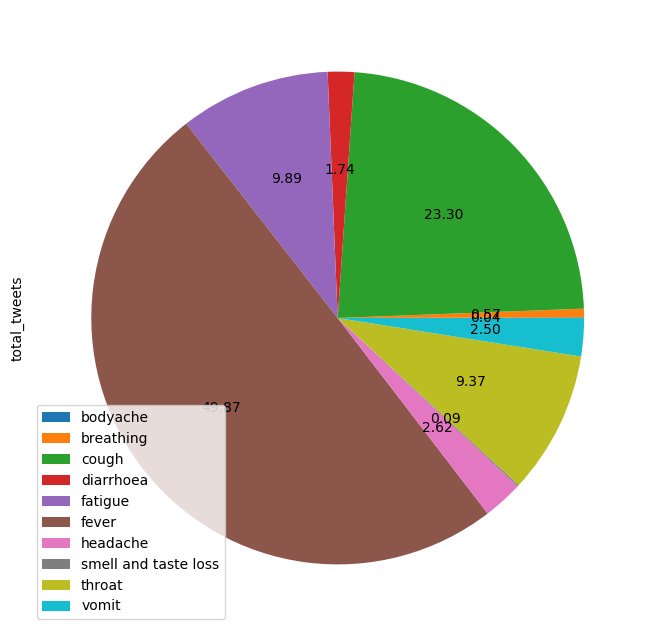
\includegraphics[scale=0.4]{city_analytics/georesults/symptoms_total_sa4.png}
    \caption{Most common symptoms}
    \label{fig:Most common symptoms}
    \end{figure}
    
    \subsection{Three Most Common Symptoms in Three Major Cities}
    The result shows the figures for Melbourne and Sydney are much larger than those of Perth. This satisfies the fact that the Melbourne and Sydney have larger populations than Perth. However, if we take a careful insight into the data, we found that the ratio 
    
    \[\frac{\text{number of symptoms tweets}}{\text{the population of the city}}\]
    
    \begin{figure}[H]
    \centering
    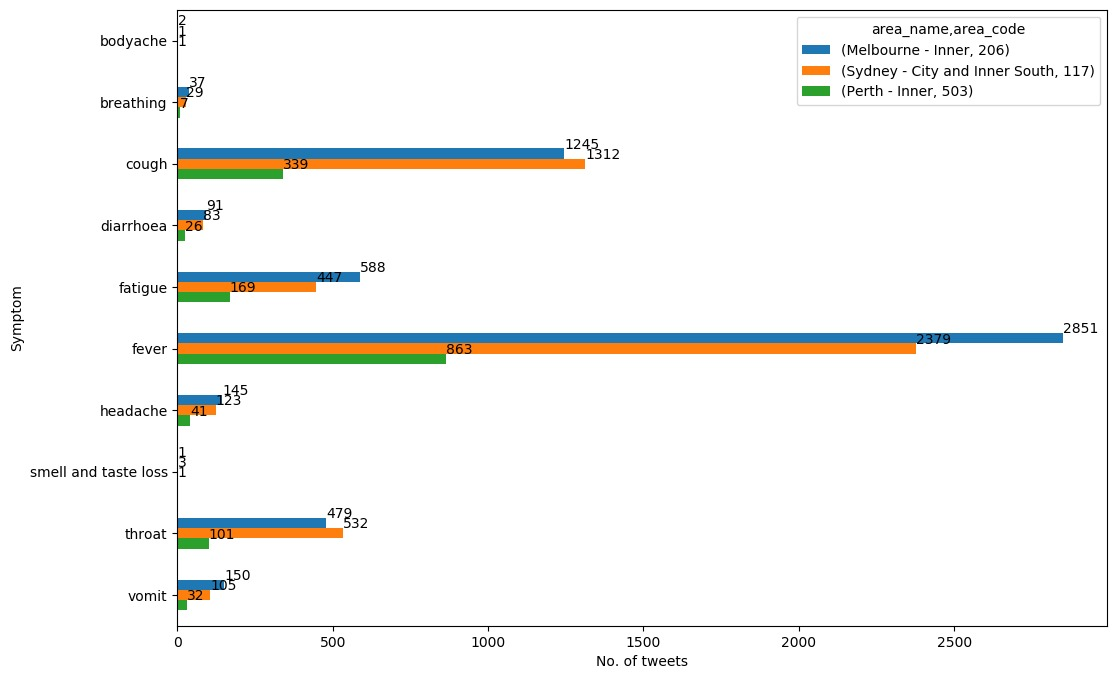
\includegraphics[scale=0.4]{city_analytics/report/images/covid-3-cities.jpeg}
    \caption{Symptoms for three major cities}
    \label{fig:Symptoms for three major cities}
    \end{figure}
    
     for Perth is much smaller than the ratios of Melbourne and Sydney, Which implies Perth has a better control of the virus than Sydney and Melbourne. Reason for that might because Perth has less population density, much less confirmed cases per million people compare with other two cities, as well as Perth has not only closed its international border but also closed the interstate border.
